\documentclass[11pt,twoside]{article}
\usepackage{times}
\usepackage{graphicx}
\usepackage{amssymb,amsmath,subcaption, hyperref}
\usepackage[symbol]{footmisc}
\usepackage[margin=1.0in]{geometry}
\title{WIFIS Simulation \\ of Nearby Elliptical Galaxy Observations}
\author{Miranda Jarvis}
\date{\today}

\begin{document}
\maketitle

\begin{abstract}

To test the performance of the WIFIS spectral image simulator code, I simulated an observation of a nearby elliptical galaxy using its known spectral and spatial properties. Here I present both the results of this simulation and some of the tests done on the effectiveness of the code and the quality of the images produced. The simulator uses Galfit to create the spatial light profile of the galaxy and the spectral element is added through a model spectrum. The code then simulates all of the processes that would affect an observation, including spatial and spectral blurring, sky emission and absorption, instrumental throughput and photon emission, and detector noise. The pertinent outputs are a data cube representing the sum of all of the sky observations and another which is the final sky subtracted image. The galaxy we model is NGC 7562 an E2 elliptical galaxy 57.29 megaparsecs away. In this document I describe how the image in the spatial plane is constructed, the spectra used and how it is calibrated to the proper flux and how the spatial and spectral directions are combined to create an accurate data cube with the correct amount of flux. I also discuss some analysis of the final images that helps demonstrate the accuracy of the code while also illuminating the quality of data that could be obtained through a real observation with WIFIS. This analysis shows that the results of the simulation match the expected values and have the appropriate amounts of noise.
\end{abstract}

\section{The Simulation} \label{simulation}

For the purposes of this document the only portions of the simulator code that will be discussed in detail are those that construct the initial spectral image that is fed into the rest of the simulator. Some of the specific parameters used in the simulation are presented in Table \ref{param}.
\begin{table}
\centering
\caption{Set-up parameters used for simulations}
\label{param}

\begin{tabular}{|l|l|}
\hline
\bf{Parameter}&\bf{Value}\\ \hline
Seeing&2"\\
Dark Current&0.02 $e^-/s/pixel$\\
Read Noise&5$e^-$\\
QE&0.76\%\\
Thermal Emission&0.5 $photons/s/pixel$s\\
Collecting Area of Telescope&3.534$m^2$\\
Spectral Resolution&3000\\
Integration Time / Frame (sky and science)&360s\\
Number of Frames (sky and science) &10\\ \hline
\end{tabular}
\end{table}




\subsection{Modelling the Spatial Direction}
To create an image of a galaxy in the spatial plane, the simulator code creates light profile models through \emph{Galfit}\footnote{Galfit Homepage: \url{http://users.obs.carnegiescience.edu/peng/work/galfit/galfit.html} }. Although the primary use of Galfit is to fit models to images of galaxies, it can also be used as a versatile model creation code that takes a number of relatively simple and well-documented inputs to create a two dimensional FITS file of the specified galaxy image. We chose to model NGC 7562 since it is a typical nearby elliptical galaxy and has complementary optical IFU data forthcoming. For our simulation we only use the most rudimentary of the Galfit modelling parameters. I modelled NGC 7562 using its physical properties as gien in the paper `Near-infrared surface photometry of early-type galaxies''\cite{Rembold}. Namely I use a Vaulcouleurs' distribution (Sersic's law with an index of 4) with an effective radius of 22.95 arc-seconds, integrated magnitude out to one effective radius of 9.7 and an ellipticity of 0.2\footnote{the paper states that the ellipticity rises form 0.1-0.3 along the semi-major axis}. 

In order for the final image to be as correct as possible I needed a method to scale the flux spatially and the model to be large enough to avoid edge effects during convolution. The latter problem was simplest to solve. Locking the centre of the galaxy to the centre of the Galfit image, the program then takes a portion of the model to correspond to the WIFIS FOV with the centre of the galaxy at any user defined position. The model is then made so that to every side of the FOV there is a buffer region before the edge of the model. This buffer space is a free parameter, for the specific simulation outlined in this report I set the buffer on each side to be 25\% the FOV along that axis. In order to be able to later scale the flux correctly, I also made a mask for the model that zeroed out all points that did not lie within one effective radius of the galaxy, taking into account the axis ratio of the galaxy and a user defined position angle. Another important detail that had to be taken into account is that Galfit works with square pixels, so I created the model with 0.11 arc-second pixels, since this is a factor of both the 1.1 arc-second slit width and 0.44 arc-second Y pixel scale of WIFIS. Figure \ref{model} shows the model of the galaxy created by Galfit and used by our simulator. 


\begin{figure}[htbp]
\centering
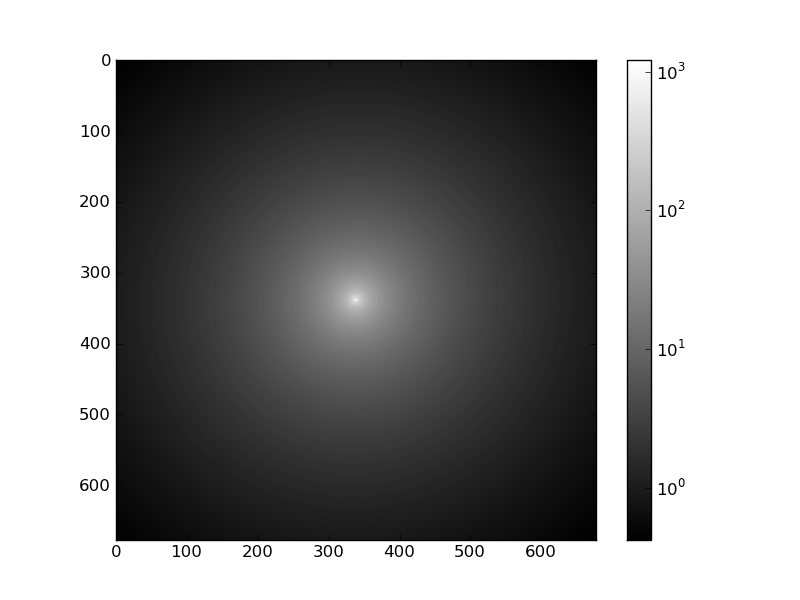
\includegraphics[width=0.75\textwidth]{galfit_model}
\caption{The model used to create the spatial profile of the galaxy for our simulation.}
\label{model}
\end{figure}

\subsection{The Spectral Dimension} \label{spectral_sect}
In order to add a spectral element to our initial image we began with a model spectrum. For running the code in general this spectrum is a free parameter as long as the units and format are correct. For my simulation of NGC 7562, I used the spectrum of a 3 Gyr elliptical galaxy with solar metalicity and Chabrier IMF created using the CvD12 model. First I ensured the spectrum had wavelength in units of nm and flux density in units of J/s/$\mu$m/m$^2$. To give the spectrum the right flux, I scaled the entire model spectrum by a constant determined by the J-band magnitude of the galaxy out to one effective radius. First I found the theoretical J-band flux based off of the J-band magnitude taken from Rembold et al\cite{Rembold}  using the following equation: \begin{equation} F_{source}=\frac{F_{vega}}{10^{m/2.5}} \end{equation} where $F_{source}$ is the flux expected in the J-band in units of J/s/m$^2$/$\mu$m, $F_{vega}$ is the flux of Vega in the J band (3.01$\times 10^{-9}J/s/m^2/\mu m$)\footnote{source of Vega Flux: \url{http://irtfweb.ifa.hawaii.edu/IRrefdata/iwafdv.html}} and $m$ is the J band magnitude of the source. I then calculated what the J-band flux was in the model spectrum. Since the spectrum was given in flux density the total flux was found by taking the mean of the flux  over the J band. By calculating the ratio between the flux found from the input spectrum and the theoretical flux of the object I scaled the whole model spectrum to the appropriate amount. Each element of the spectrum now contained the integrated flux out to one effective radius of the galaxy for that wavelength. The next paragraph describes a test of how well this spectrum fits observations, after that I describe how the spectrum created here was manipulated for use in the final simulation.

To ensure both that the model spectrum we used had the right general shape, and that our scaling had created reasonable flux values, I then compared the spectrum I had created with those given in ``Infrared Spectroscopy Of Nearby Radio Active Elliptical Galaxies''\cite{Mould}. First of all I converted the flux into units of $ergs/s/\AA/cm^2$, then I had to scale the spectrum to correspond to the a 1 arc-second slit used to observe the galaxies in the paper. Firstly, by summing over all the wavelengths in the spectrum I got a value for the total flux from the galaxy out to one effective radius ($F_R$). I then used the mask created earlier to calculate the flux in the Galfit model out to one effective radius ($F_{elps}$), then used the ratio $F_R/F_{elps}$ to scale the model so that it contained the appropriate amount of flux. Since I only needed to consider the flux contained in a 1 arc-second slit for this test I summed the model over a 1.1 arc-second region (closest integer number of pixels) which I then estimated as having 1\% too much flux so I subtracted out 1\%, I then used this value to scale the spectrum after normalizing it first. The resulting spectrum is shown in Figure \ref{compspec} along with the observed spectrum of an elliptical galaxy \cite{Mould}.

\begin{figure}[htbp]
\centering  
\begin{subfigure}{0.5\textwidth}
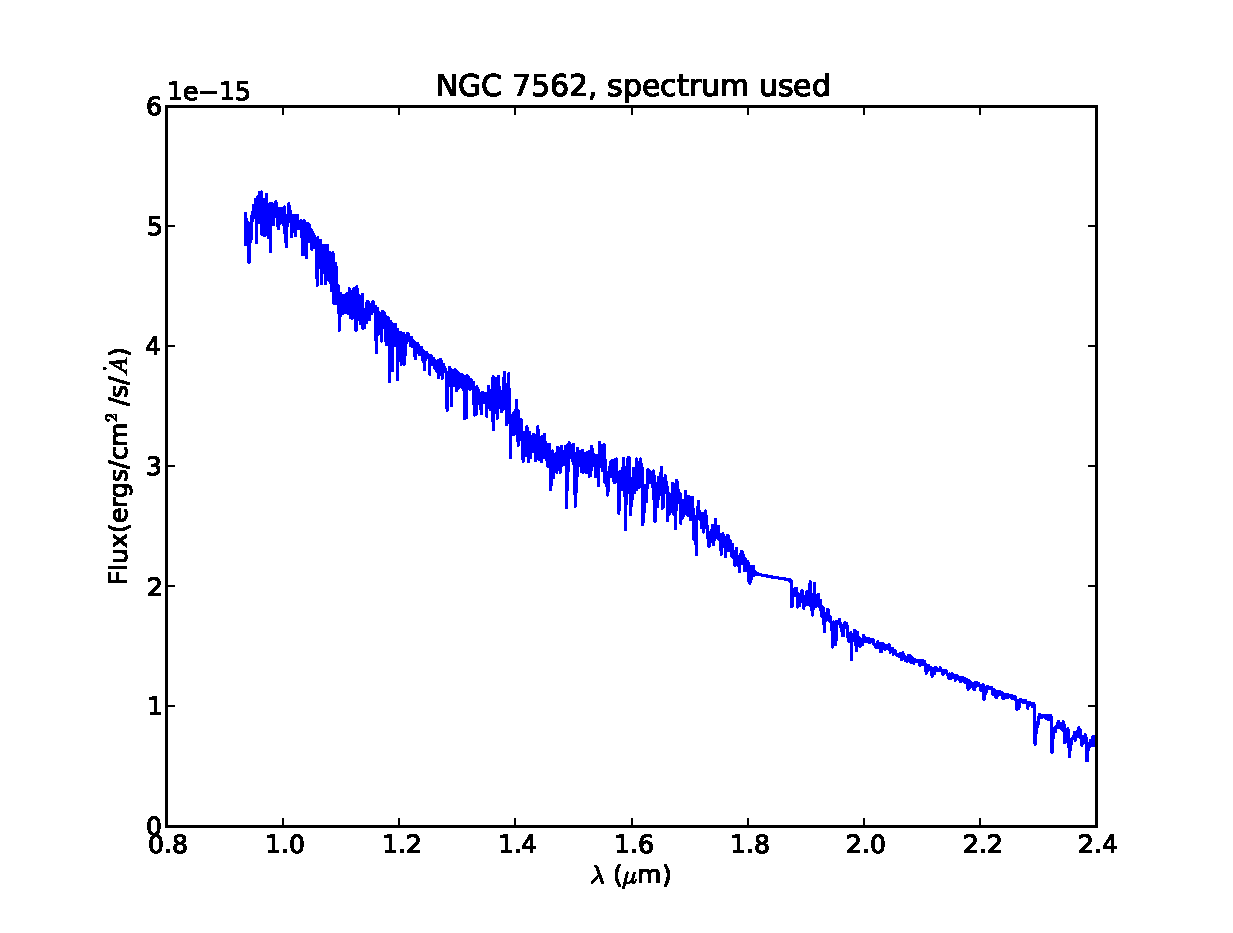
\includegraphics[width=0.99\textwidth]{flux_for_slit_comp}
\caption{rescaled spectrum of NGC 7562 based on model}
\end{subfigure}%
\begin{subfigure}{0.5\textwidth}
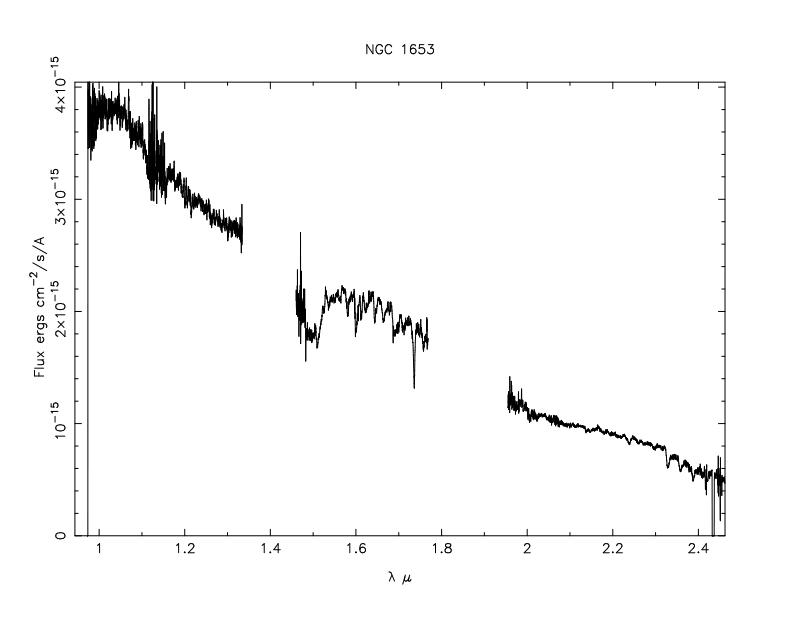
\includegraphics[width=1.1\textwidth]{spec_compare}
\caption{one of the spectra from the data set in Mould et al (2012)}
\end{subfigure}
\caption{Comparing the model spectrum created for our simulation with real observations. The overall shape and many of the large scale features appear in both.}
\label{compspec}
\end{figure}

In order to create the final spectrum used to create the model data cube for the simulator I convolved the spectrum and changed the pixel scale to that of WIFIS by taking the integral of the flux density spectrum over each WIFIS pixel range.  By multiplying by $\lambda/(h*c)$ I converted from energy flux to photon flux.

\subsection{Creating the Data Cube and Flux Conservation}\label{flux_sec}
Now I had two distinct parts: the Galfit model and the flux calibrated two dimensional spectrum. There are many ways in which I could have put these together into a two dimensional data cube. I chose the method described below to save on computation time. The main issue is that the Galfit model is at a finer pixel scale than WIFIS, and so needs to be re-binned which is much faster to do in 2D. The first few steps in producing the data cube are similar to that explained in section \ref{spectral_sect}. Looking only at the portion of the spectrum within WIFIS' spectral range I found $F_R$ then found the flux in the model out to the effective radius using the mask  so that I could scale the entire Galfit model by $F_R/F_{elps}$ .  I then convolve the image with the psf: a gaussian with a standard deviation defined by the seeing (2'' in this case). I convolve at this point in the simulation to avoid edge effects degrading the image quality. The next step is to crop the image to include only the WIFIS field of view and re-bin to the right pixel scale. Now the spectral direction can be added in. After normalizing the spectrum by dividing by its sum I created a data cube with the normalized spectrum along the spectral direction of each pixel I then multiplied in the model to add the appropriate flux at each spatial pixel. Table \ref{flux} shows how the flux is carried throughout these steps as well as how the flux is conserved through the rest of the simulation. The flux is conserved almost perfectly throughout all steps except the flux recovered from the end of the simulation which suffers from statistical variation due to noise. The recovered flux for a single simulation varied by a maximum of 0.01\% for the 10 runs of the simulation that I calculated the final flux for, however the mean of the 10 values was only off by 0.001\% with an error in the mean of 18.

\begin{table}[htbp]
\centering
\caption{The total flux in various stages of the simulation. Stage 1 is the theoretical integrated flux to one effective radius. Stage 2 the sum of the portion of the model out to one effective radius after having been scaled to the appropriate flux, and stage 3 has been convolved to the seeing. Stage 4 is the total flux in the WIFIS FOV (it is different because a different region is being considered), then stage 5 has been re-binned to the WIFIS pixel size. Then the spectrum is added in stage 6 creating a data cube. Stage 7 is the mean of total flux in the reduced data cubes of 10 runs of the simulation and the associated error in the mean.}
\label{flux}
\begin{tabular}{|l|l|}
\hline
\bf{Stage}&\bf{Flux (photons/sec/m$^2$)}\\ \hline
1)&1145700\\
2)&1145700\\
3)&1145700\\
4)&927590\\
5)&927590\\
6)&927590\\
7)&927600$\pm18$\\

\hline
\end{tabular}
\end{table}



\section{Analysis}
After simulating the observations, I analyzed the files created to assess both the effectiveness of the simulator and the quality of the images produced. I focused on two regions of the images for this analysis, one centred on the core of the galaxy and one close the the edge of the field of view. I used the width of the typical seeing at the Kitt Peak site (2 arc-seconds) to define the size of the boxes, taking into account the pixel scale in each direction, creating a rectangle 4 pixels wide in the X direction and 5 in the Y where Y is the long axis on our FOV. Figure \ref{final} shows the final sky subtracted image produced by the simulator summed over all wavelengths with the two apertures considered outlined in white.

\begin{figure}
\centering
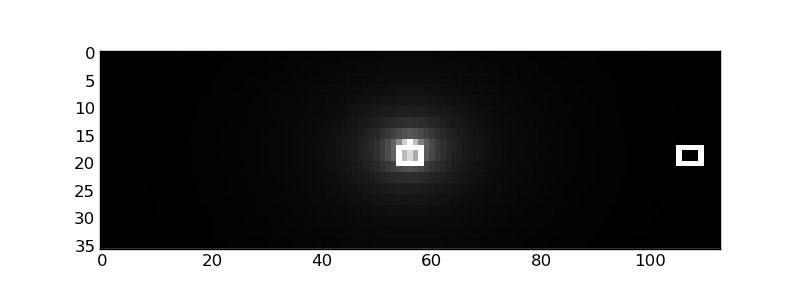
\includegraphics[width=\textwidth]{final_img}
\caption{The results of the simulator code summed over the entire spectral range with the two apertures used over plotted in white, one centred on the glalaxy the other on the edge of the frame.}
\label{final}
\end{figure}

\subsection{Reducing the Simulated Spectrum}
The simulator code produces a final data cube that is a sky subtracted image with the appropriate noise. However, there is no built in correction for telluric or instrumental effects on the shape of the spectrum. In order to compare the original and final flux values as I did in Section \ref{flux_sec} these effects had to be removed. To do this I divided the spectrum by the sky transmission and instrument throughput values used in the simulator, as well as by the telescope collecting area. I then compared this to the spectrum on the same region from the unmodified data cube created in section \ref{simulation}. Figure \ref{rspec} compares the reduced spectrum from the simulation and the origional, each spectrum shown is the mean over the respective aperture.

\begin{figure}[htp]
\centering  
\begin{subfigure}{0.5\textwidth}
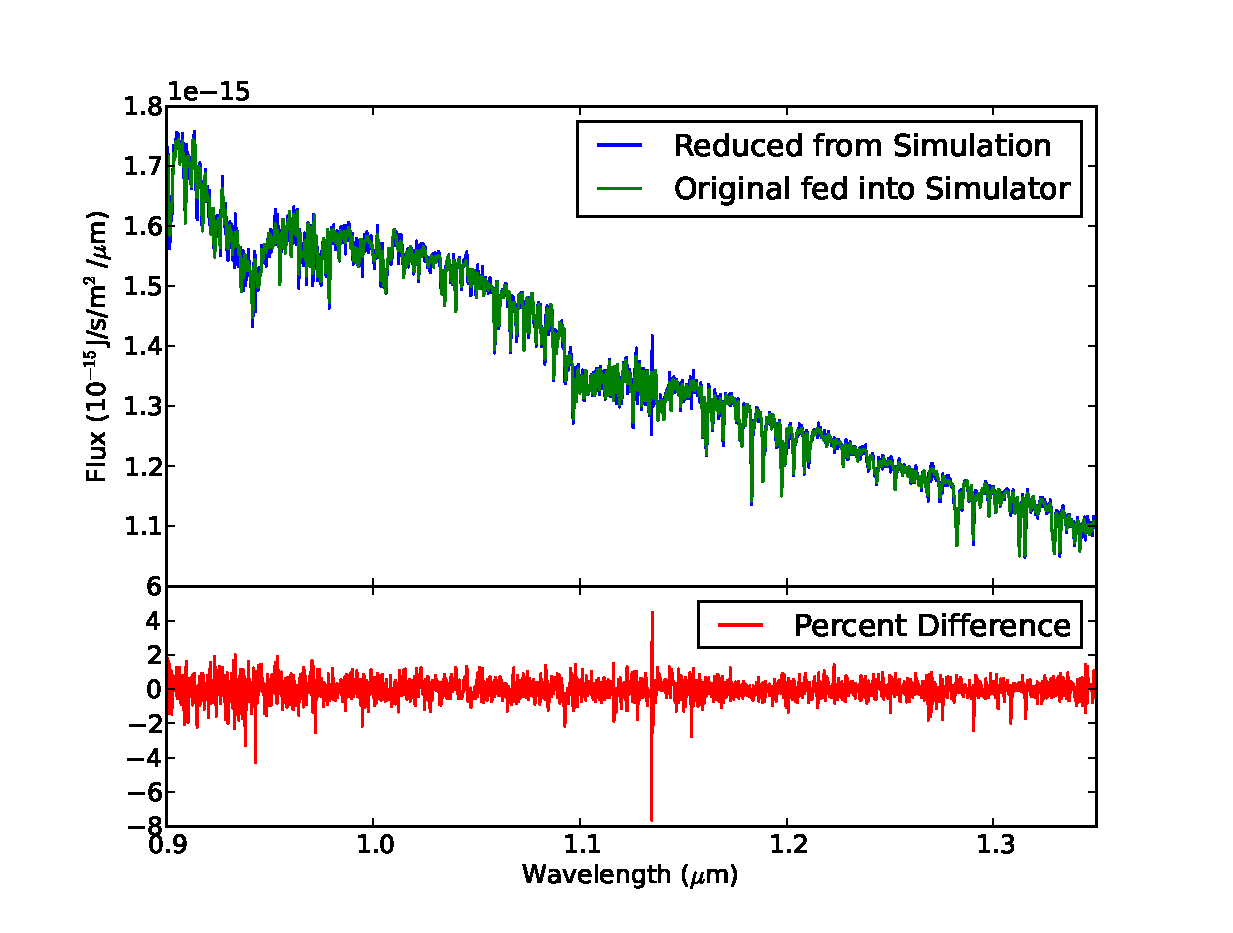
\includegraphics[width=\textwidth]{reduced_spect}
\caption{ The mean spectrum from the aperture centred on the galaxy core.}
\end{subfigure}%
\begin{subfigure}{0.5\textwidth}
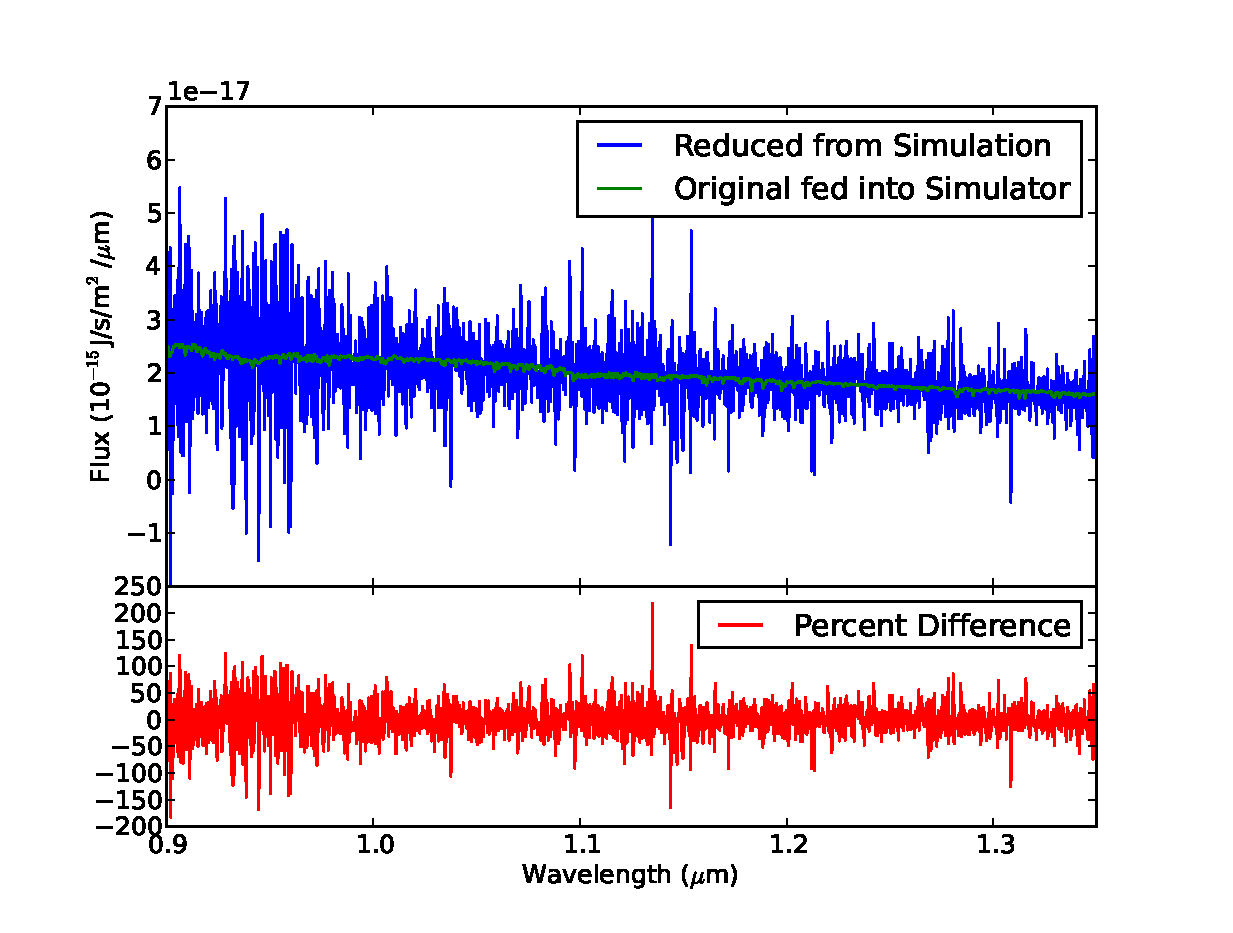
\includegraphics[width=\textwidth]{reduced_spect_edge}
\caption{The mean spectrum from the edge of the FOV.}
\end{subfigure}
\caption{Comparing the spectrum recovered from the simulator to that from the initial data cube for both apertures. Each has been converted to units of energy flux density.}
\label{rspec}
\end{figure}


\subsection{Signal to Noise Calculations}
One of the most important steps in determining the quality of an image is computing the signal to noise ratio (S/N). As part of the image analysis for my simulator, I have calculated the signal to noise in two distinct ways: one using the final data cubes produced by the simulator, the other using the theoretical values used in the simulation. 

The first method is meant to simulate how the signal to noise would be found from a `real' observation. The main challenge with calculating the signal to noise from the simulated observations (as it would be for a real observation of a similarly sized galaxy with WIFIS) is that the source extends to the edges of the field of view so nowhere in the final reduced image can be considered to contain only noise. So in order to calculate the signal to noise from the simulated images I used the sky frame as well as the sky subtracted science image. For each wavelength slice I calculated the standard deviation of the sky frame using the equation: \begin{equation} \sigma_{sky}=\sqrt{\overline{x^2}-\bar{x}^2} \label{skyerr}\end{equation} where $\sigma_{sky}$ is the standard deviation of a single pixel, x is the flux values of the sky image at a given wavelength and the bar implies taking the mean. This value takes into account all of the noise sources in the sky image, namely poisson noise from the sky emission, thermal emission and dark current as well as read noise. To find the standard deviation for the entire aperture we take $\sigma_{sky}\sqrt{n}$ where $n$ is the number of pixels in the aperture. To account for the fact that the final image is actually the science frames minus the sky frames we also need to consider the noise in the science frames. The science frames have the same noise sources as the sky frames only they also have poisson noise from the source. It is also worth noting that the data cubes produced by the simulator are in units of electrons/s. Since in our simulation we take the same number of science and sky frames at the same integration time we are able to simply consider $\sigma_{sky}$ twice in our final noise equation. The source noise ($\sigma_{source}$) can be calculated using the sum of the final sky subtracted image in the aperture, call this value $S$ (the source value), as: \begin{equation} \sigma_{source}=\frac{\sqrt{S}}{\sqrt{t*n_i}} \end{equation} where $t$ is the integration time of one frame and $n_i$ is the number of frames used. In our case both the science and sky images were compose of 10 six minute exposures. The final noise is then calculated as \begin{equation}N=\sqrt{2n\sigma_{sky}^2+\sigma_{source}^2}\end{equation}

 I also calculated the signal to noise using the theoretical values, this method closely parallels the equations used to add the noise in the simulator. For the source value (S) I take the data cube of the target before the sky emission has been added or noise applied and find the sum of that array over the aperture for each wavelength. I then calculated theoretical noise in both the science frame and sky frame using the following equations: 
\begin{equation} \sigma_{sci}=\frac{\sqrt{((S+(d+thm+sky)n)t_{sci}+r^2n)n^i_{sci}}}{t_{sci}n^i_{sci}} \label{noise1}\end{equation} and \begin{equation} \sigma_{sky}=\frac{\sqrt{((d+thm+sky)nt_{sky}+r^2n)n^i_{sky}}}{t_{sky}n^i_{sky}} \label{noise2}\end{equation} where $t_{sci}$ and $n^i_{sci}$ and are the integration time and number of science frames, similarly for the sky; then $d$ is the dark flux, $thm$ is the thermal flux  and $sky$ is the sky flux at a given wavelength, each of these is per pixel per seconds hence why each is multiplied by the number of pixels in the aperture (n) as well as the integration time. Then $r$ is the read noise per integration. 
Then the noise in the final sky subtracted image is
\begin{equation}N^2=\sigma_{sky}^2+\sigma_{sci}^2 \label{noise3}\end{equation}

Figure \ref{SN} shows the results of these signal to noise calculations and compares the theoretical results to those from the simulation for both apertures. Note how the portions of Figure \ref{rspec} with the largest residuals correspond to regions of lower signal to noise. This implies that the discrepancy is due to noise, not errors in the simulation.

\begin{figure}[htp]
\centering  
\begin{subfigure}{0.5\textwidth}
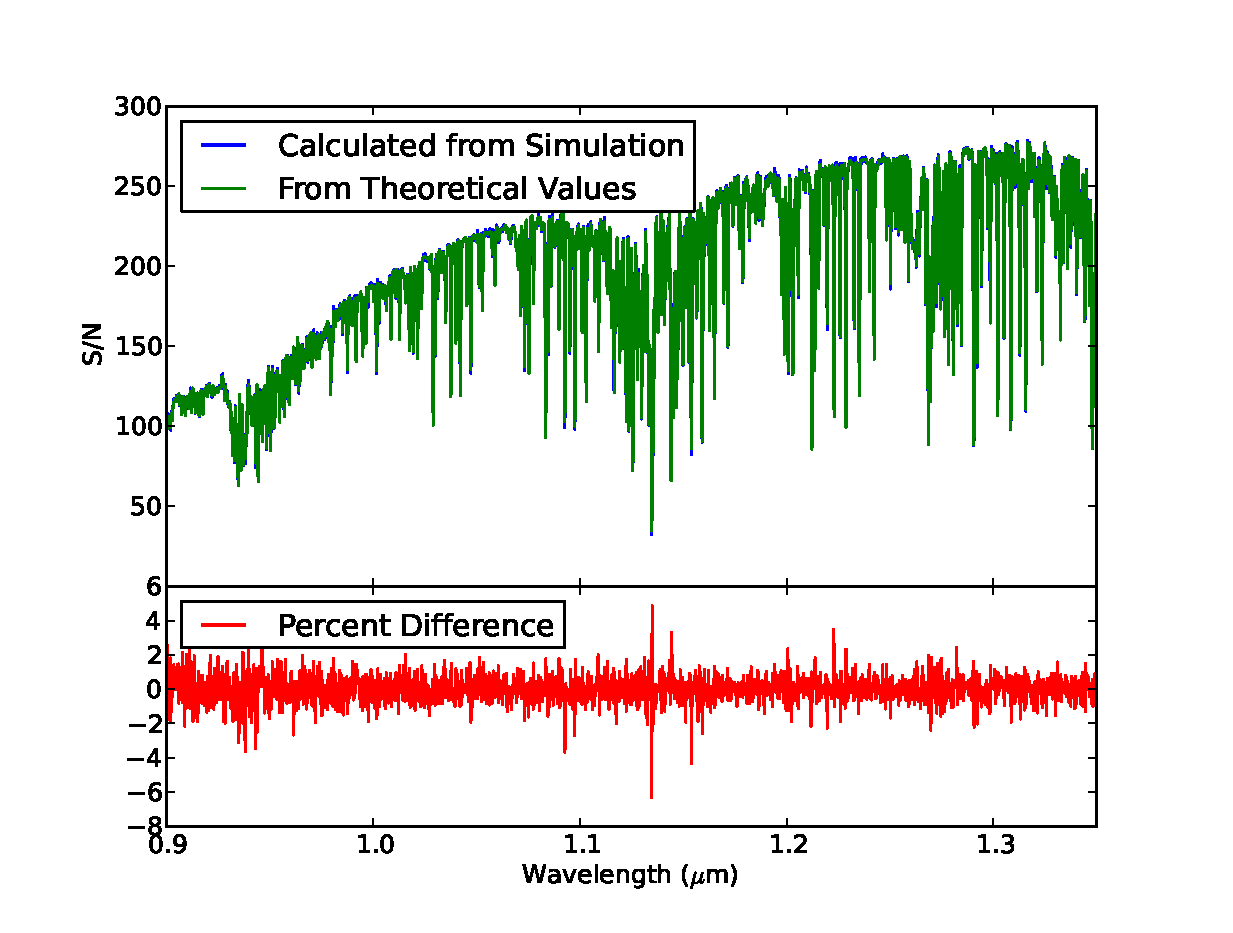
\includegraphics[width=\textwidth]{signal_noise}
\caption{The signal to noise from the aperture centred on the galaxy core.}
\end{subfigure}%
\begin{subfigure}{0.5\textwidth}
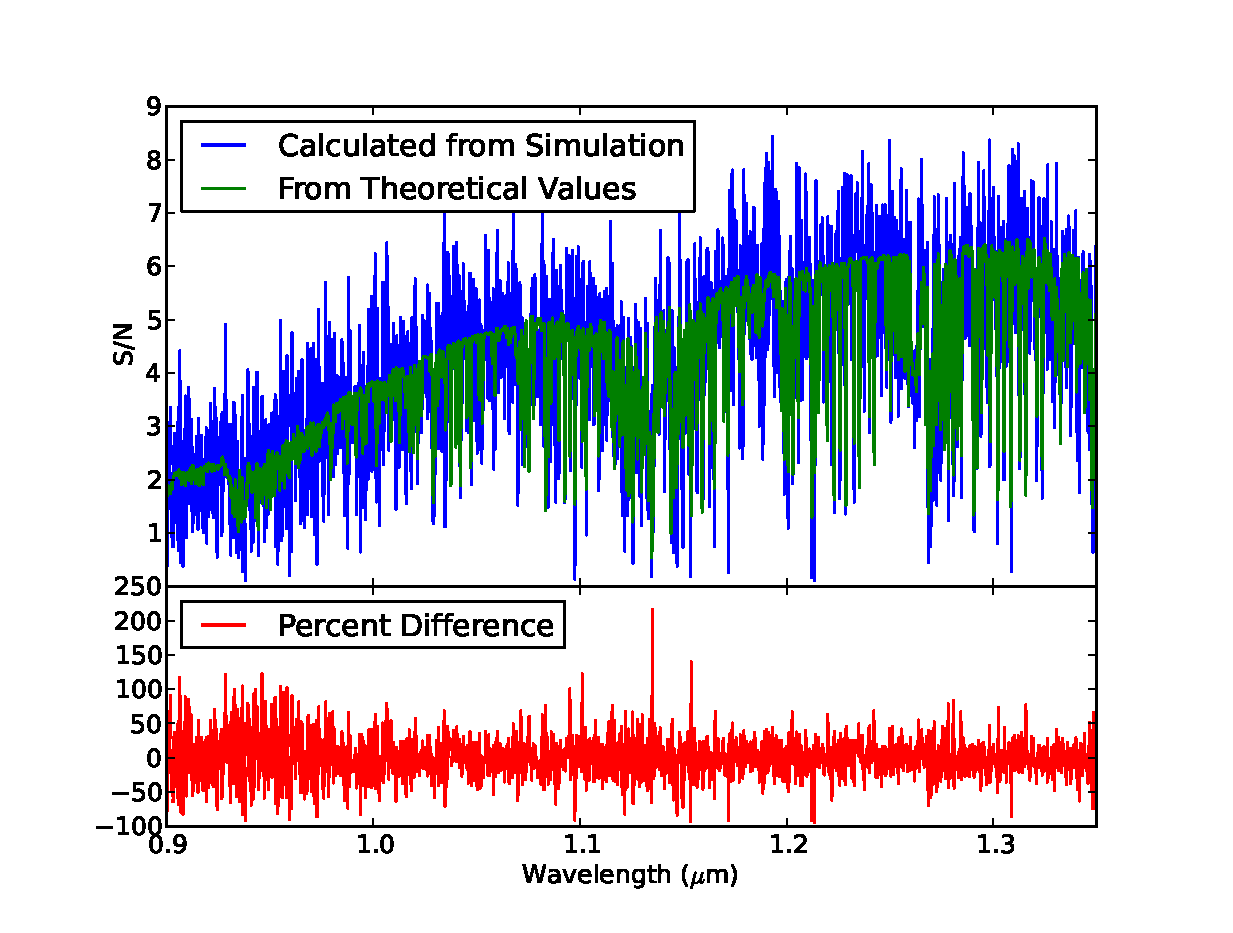
\includegraphics[width=\textwidth]{signal_noise_edge}
\caption{The signal to noise from the edge of the FOV.}
\end{subfigure}
\caption{Comparing the signal to noise calculated from the simulated observations to theory for both of the apertures.}
\label{SN}
\end{figure}

I also consider the possible improvement in signal to noise from re-binning the images. Since our pixel size in both spatial directions is smaller than the expected seeing by about a factor of two, re-binning such that each new pixel contains two of the original in each direction does not lose any spatial information, it does however result in a significant improvement in the S/N for an individual pixel. Figure \ref{bin} shows the signal to noise for a single pixel from the original images produced by the simulator compared to that for re-binned images. The Signal to noise in each case is found using the first method described above at the centre of the image, and for the un-binned case the value shown is the mean of four pixels.

\begin{figure}[htp]
\centering
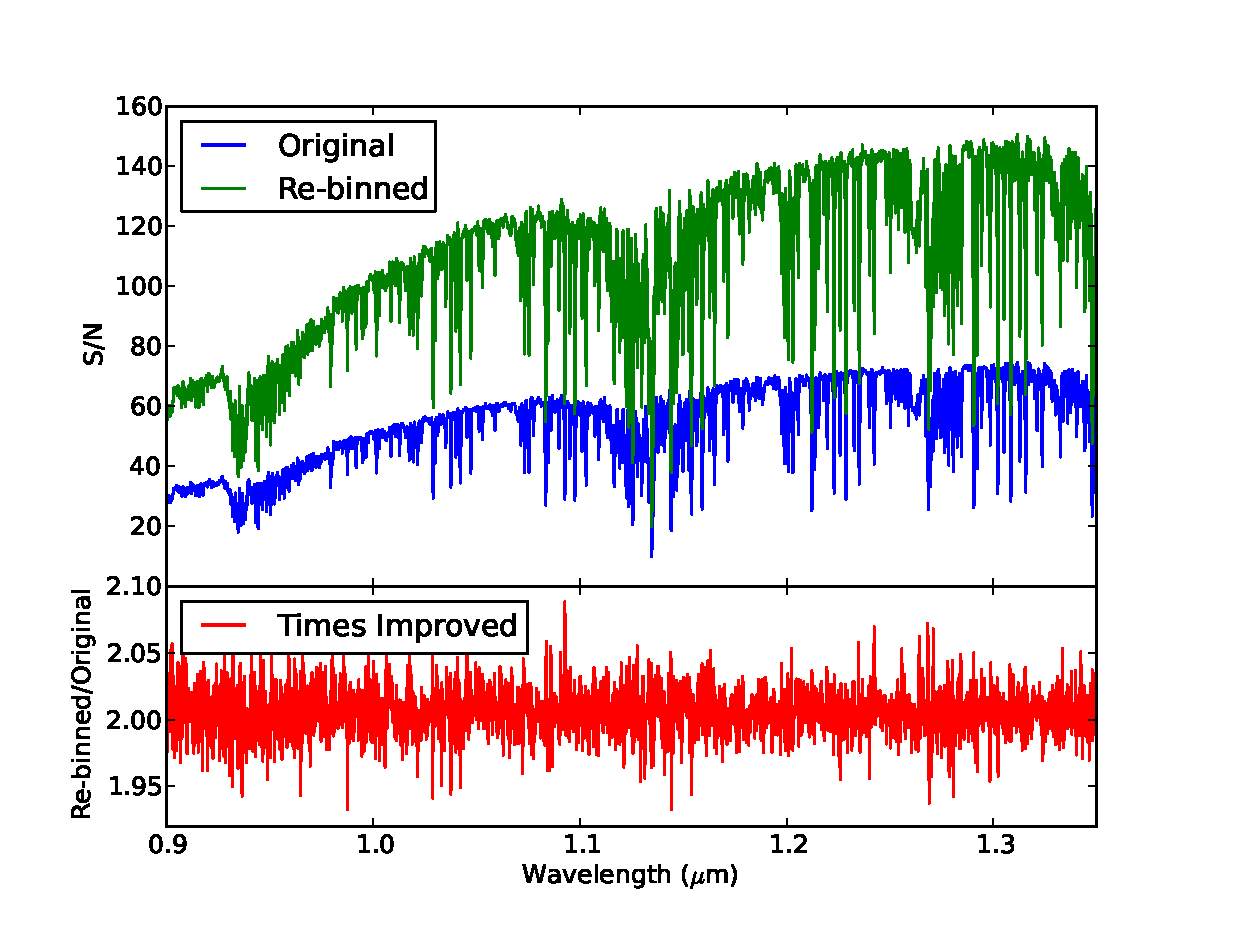
\includegraphics[width=0.75\textwidth]{SN_rebin}
\caption{Improving the signal to noise per pixel by re-binning the simulated images in the spatial plane so each pixel is 2X2 original pixels wide.}
\label{bin}
\end{figure}


\subsection{Relative Contribution of Various Noise Sources}
For all of the noise calculations I have done above, I have attempted to be as exact as possible, considering all sources of noise. However often during real image analysis simplifications are made to calculate signal to noise, for example ignoring the Poisson noise from the source. For this reason and to discover which noise source are dominant, I decided to compare the relative influences of the various sources of noise in our simulations. For the signal I used the mean pixel value of each aperture from the pre sky and noise image. I calculated the total noise at each wavelength using equations \ref{noise1}-\ref{noise3} with $n=1$ since we are only considering one pixel. I then split the noise equation up by source: \begin{equation} N^2=N_S+N_{sky}+N_{thm}+N_d+N_r \end{equation}
$N_S$ is the source noise and is found using \begin{equation} N_S=\frac{S}{t_{sci}n^i_{sci}}\end{equation} using the same variable definitions as in equations \ref{noise1} and \ref{noise2}. $N_{sky}$, $N_{thm}$ and $N_d$ all have very similar equations where $N_x$ and $x$ represent each of them respectively: \begin{equation} N_x=\frac{x}{t_{sci}n^i_{sci}}+\frac{x}{t_{sky}n^i_{sky}} \end{equation} and $N_r$ is read noise, calculated by \begin{equation} N_r= \frac{r^2}{t_{sci}^2n^i_{sci}}+\frac{r^2}{t_{sky}^2n^i_{sky}} \end{equation} I then calculated the percent contribution of each noise source by dividing the value of each individual noise by the total noise. The results are shown in Figure \ref{relnoise}. The source noise is quite significant near the core but negligible near the edge of the FOV.

\begin{figure}[htp]
\centering  
\begin{subfigure}{0.5\textwidth}
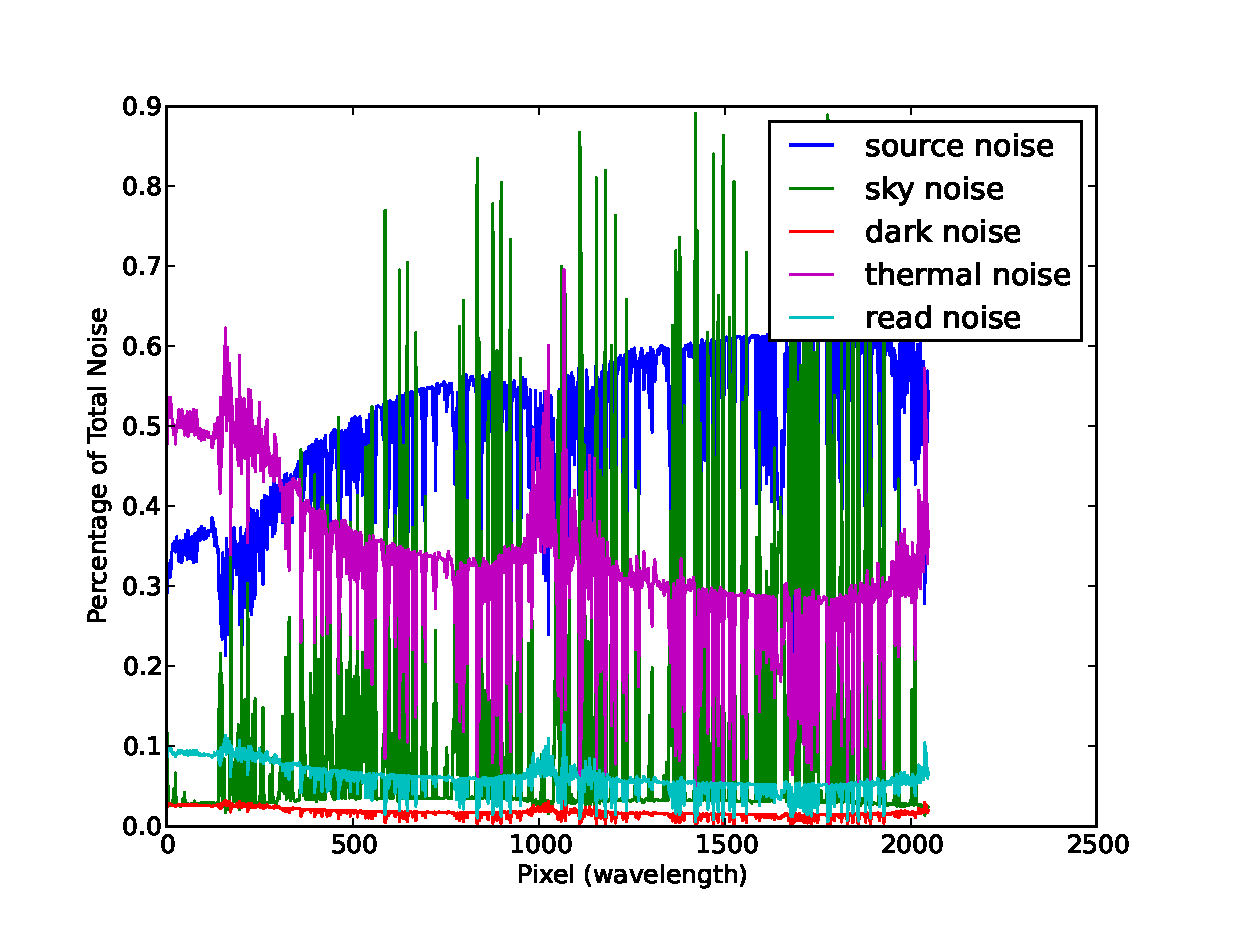
\includegraphics[width=\textwidth]{noise_comp}
\caption{The relative influence of the various noise sources from the aperture centred on the galaxy core.}
\end{subfigure}%
\begin{subfigure}{0.5\textwidth}
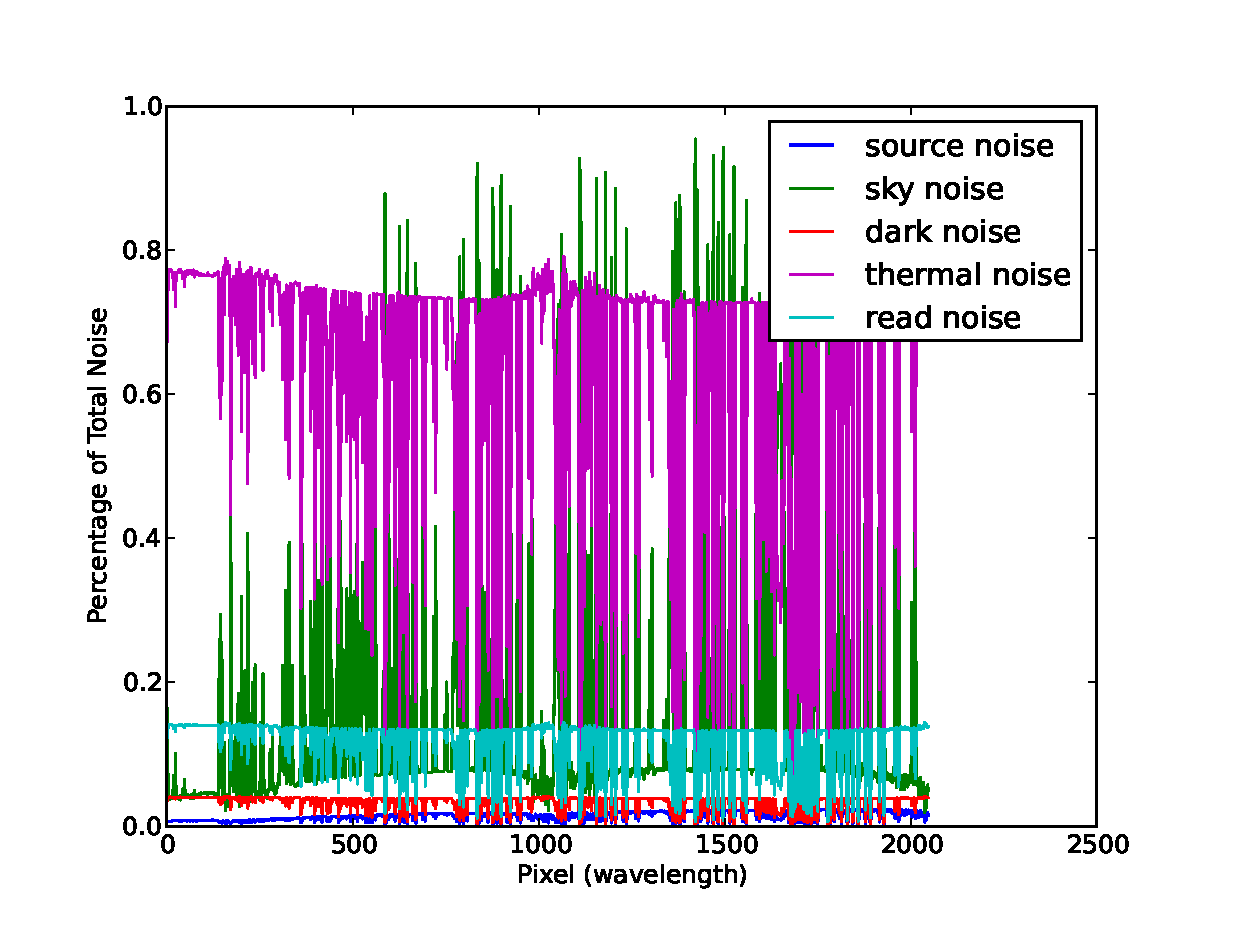
\includegraphics[width=\textwidth]{noise_comp_edge}
\caption{The relative influence of the various noise sources from the edge of the FOV.}
\end{subfigure}
\caption{How each of the noise sources in our observation impacts the final image depending on position on FOV considered.}
\label{relnoise}
\end{figure}

\subsection{Detection Sensitivity}

To get a better idea of the effectiveness of the instrument and as a further test of the simulator, the flux needed for a ten $\sigma$ detection was also calculated. In order to compare properly with instrument performance predictions I calculated the sensitivity by simulating an observation with no source. In a real observation this could similarly be done by finding the reduced spectra shown in Figure \ref{rspec} for the sum over each aperture instead of the mean and then dividing it by  the signal to noise in Figure \ref{SN}, then multiplying by 10 for 10 $\sigma$. For the zero source case however it was much simpler. For each wavelength I used the final sky subtracted image from the simulator and calculated the standard deviation using all of the pixels at that wavelength as `x' in equation \ref{skyerr}, then also like the sky noise above, I multiplied by the square root of the number of pixels in the aperture, finally I multiplied by 10 to find the flux needed at each wavelength for a 10 $\sigma$ detection. After dividing by the collecting area, the throughput of the telescope and sky transmission I had the amount of flux necessary from the target. Finally I converted from photons/s/m$^2$ to erg/s/cm$^2$. For real observations however source noise would have effect as well and cause larger values for the sensitivity. The values I found can be compared to performance predictions. Figure \ref{sensitive} shows the zero source detection sensitivity I calculated from my simulations as well as theoretical predictions made by Suresh Sivanandam.

\begin{figure}
\centering
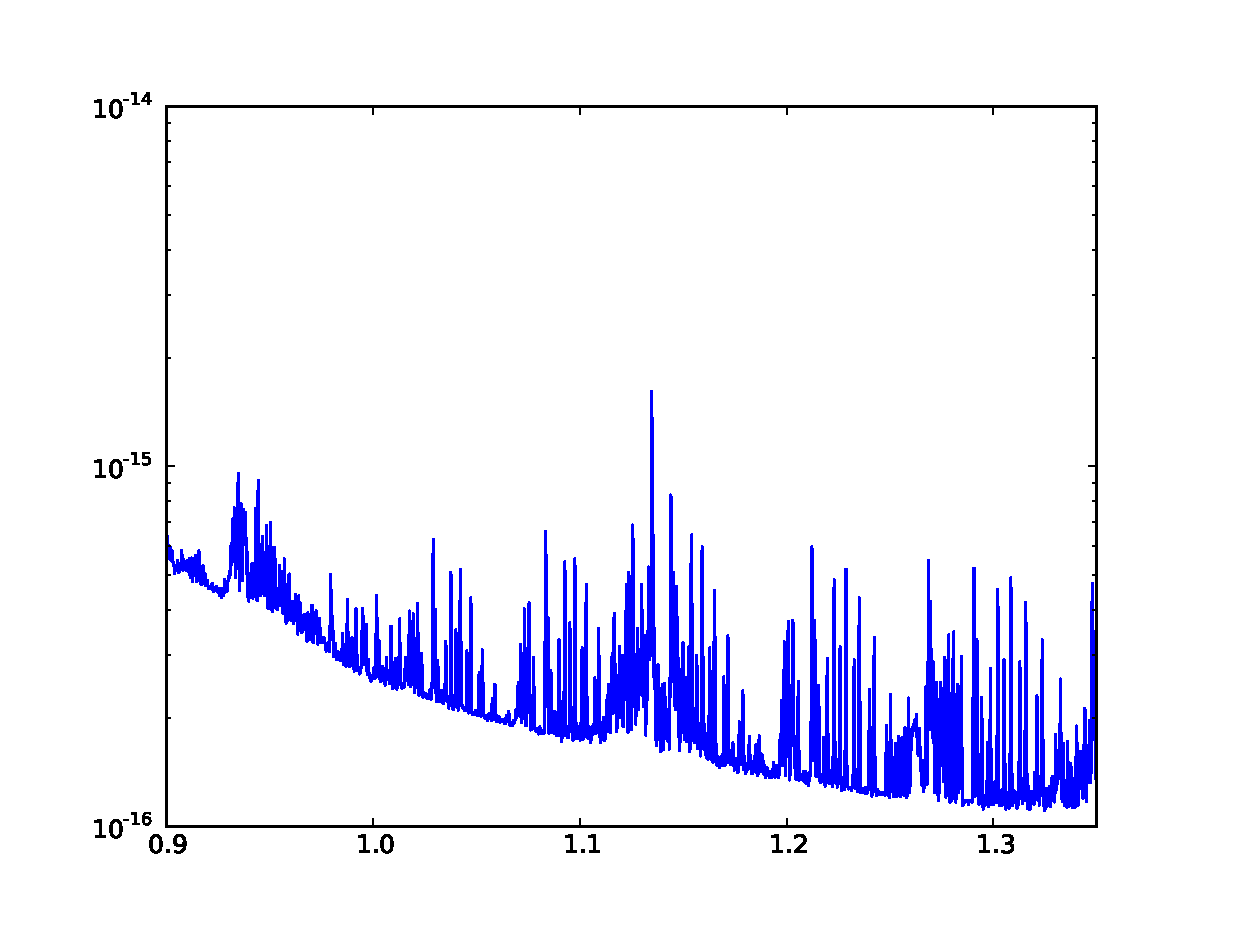
\includegraphics[width=0.75\textwidth]{nosource_sensitivity}
\caption{Simulated detection sensitivity for a ten $\sigma$ detection on an aperture as wide as the seeing (2'')} 
\label{sensitive}
\end{figure}



\section{Conclusion}
The spectral image simulator for WIFIS seems to be preforming admirably. It is able to create accurate models of elliptical galaxies given a sample spectrum and morphological parameters and from that predict what the galaxy will look like if imaged by WIFIS. The quality of the simulations themselves is also good. The initial spectrum is able to be retrieved with reasonable accuracy limited seemingly only by the signal to noise, which itslef matches the theoretical values for these observations. In the future I would like to be able to use simulated observations of a reference star to reduce the spectrum and produce simplified models of spiral galaxies to simulate as well. Based off of the tests outlined above as well as some more basic tests already preformed, including checking the convolution widths and noise intensity of the images, it seems that the simulator is able to produce high quality images, accurately depicting the performance of WIFIS.

\begin{thebibliography}{9}



\bibitem{Mould}
Mould, Jeremy; Reynolds, Tristan; Readhead, Tony; Floyd, David; Jannuzi, Buell; Cotter, Garret; Ferrarese, Laura; Matthews, Keith; Atlee, David; Brown, Michael. ``Infrared Spectroscopy of Nearby Radio Active Elliptical Galaxies'' The Astrophysical Journal Supplement, Volume 203, Issue 1, (2012). Data available at \url{https://sites.google.com/site/radioactivegalaxies/home/test}.

\bibitem{Rembold}
Rembold, S. B.; Pastoriza,  M. G.; Ducati, J. R.; Rubio, M.; Roth, M. ``Near-infrared surface photometry of early-type galaxies''. A\&A 391, 531.545 (2002)


\end{thebibliography}
\end{document}
